\normaltrue \difficilefalse \tdifficilefalse
\correctionfalse

%\UPSTIidClasse{11} % 11 sup, 12 spé
%\newcommand{\UPSTIidClasse}{12}
% CCP MP 2014
\exer{Escalier mécanique$\star$ \label{A3:01:60}}
\setcounter{numques}{0}
\UPSTIcompetence[2]{A3-01}
\index{Compétence A3-01}
\index{Escalier mécanique}
\index{Associer les fonctions aux constituants.}

\ifcorrection
\else
\textbf{Pas de corrigé pour cet exercice.}
\fi

\ifprof
\else


Un escalier mécanique (figure 1), appelé aussi escalier roulant ou Escalator (nom déposé par la société Otis), est un élévateur adapté au transport de personnes. Sa fonction principale est de faciliter le déplacement des piétons entre deux points de différentes hauteurs. 

%Depuis son invention en 1892 (à New York) par l’américain Jesse W. Reno, le système n’a pas cessé d’évoluer pour s’adapter aux nouvelles contraintes économiques, environnementales et sécuritaires.


\begin{figure}[H]
\centering
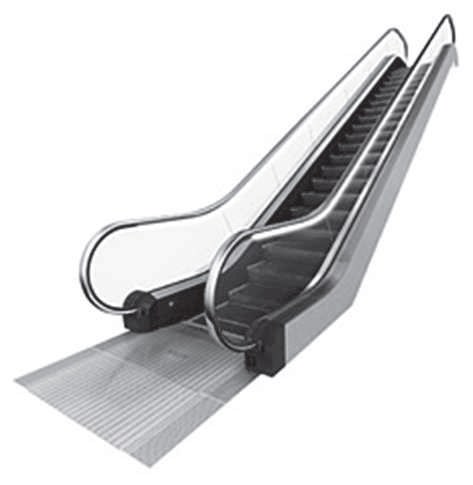
\includegraphics[width=4cm]{60_01}
%\caption{Amplificateur de charge à plusieurs canaux KISTLER. \label{fig_50_01}}
\end{figure}

%\ifprof
%\else
%\end{multicols}
\begin{figure}[H]
\centering
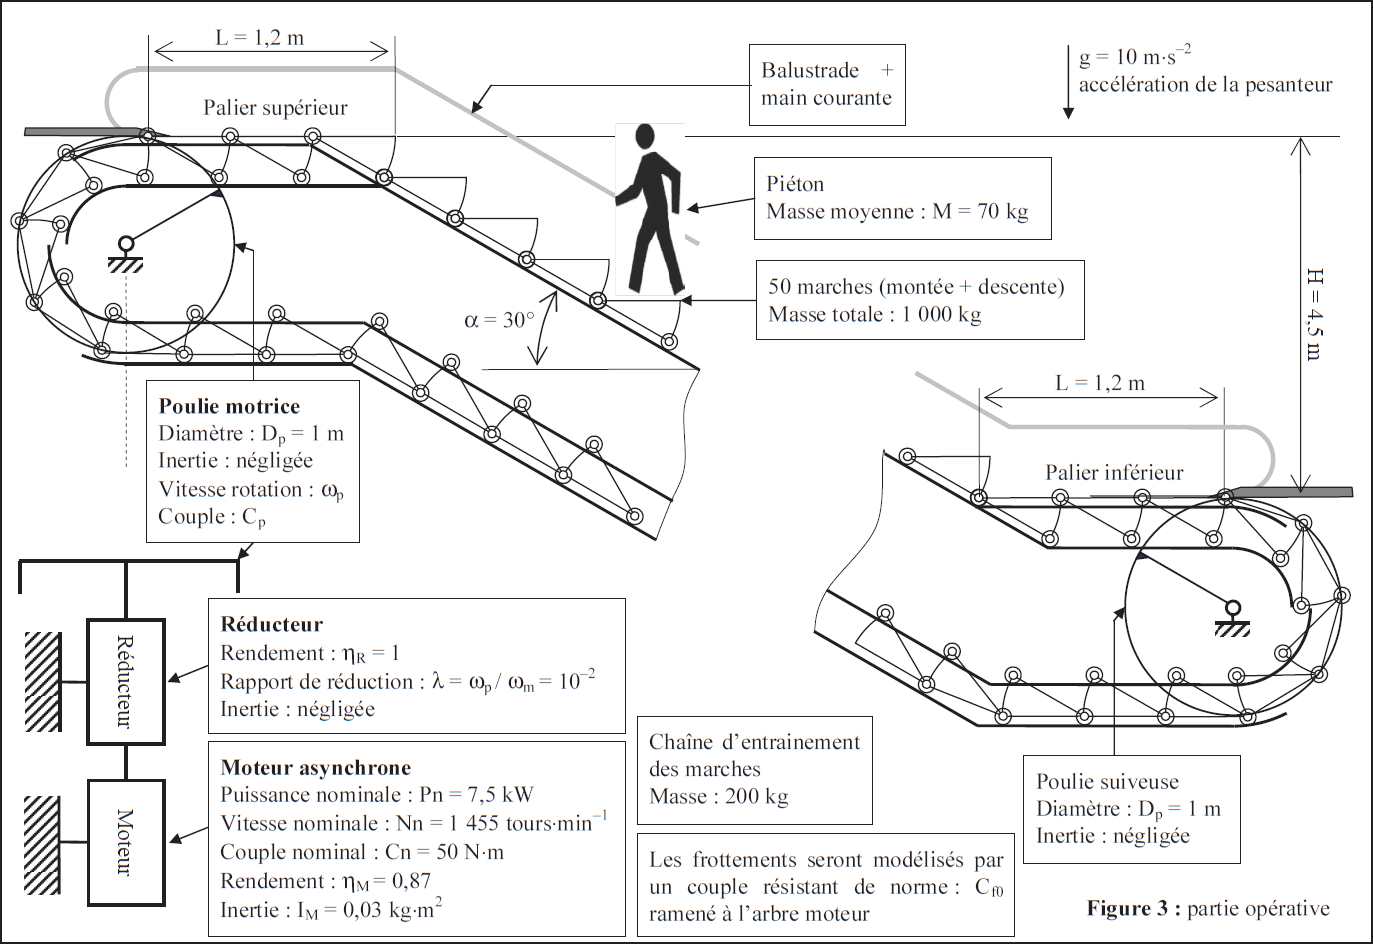
\includegraphics[width=\linewidth]{60_02}

\end{figure}
%\begin{multicols}{2}
%\fi




\question{En analysant le schéma de principe de la figure précédente, proposer une chaîne fonctionnelle de l'escalier mécanique.}


\ifprof
\else
\begin{flushright}
\footnotesize{Corrigé  voir \ref{A3:01:60}.}
\end{flushright}%
\fi